\section{Results \& Discussion}
In this section, we present and compare the results gathered from all experiments at sub-microscopic modeling level. Each task allocation run, for a team of 5 robots placed in a 160X160 arena, lasted 3 minutes (simulated time) and 40 runs were carried out for each simulation setup. The colored bars stand for the average performance and the error bars represent the standard deviations among runs. Different parameters were tuned for each case scenario and are described in the subsequent subsections. Furthermore, unless otherwise stated, our stimuli were the number of pixels (from the processed image) corresponding to the closest task (cylinder) for each color.

\subsection{Performance Metrics}
The purpose of this project is to assess the benefit of dynamic, or adaptive, thresholds-based algorithms over static ones (whether it be the homogeneous or heterogeneous case). To do so, we introduce two performance metrics:
\begin{itemize}
	\item The number of tasks processed within a time period ($N/T$)
	\item One minus the distance traveled per processed task \\ ($1-d/N$)
\end{itemize}  
Since it is better to travel less per processed task, the transformation above was necessary so that all agents want to maximize those two metrics. 
While the former gives us an idea of the average rate at which actions are performed, the second embeds two notions at the same time: the distribution of workload among robots and the efficiency of the allocation in terms of distance from robots to tasks, which can be useful on real robots where the power supply is limited.

\subsection{Private Fixed-Threshold Task Allocation}
For these experiments, we compare the performances obtained for two different fixed thresholds in both deterministic and probabilistic cases. In the probabilistic case, a sigmoid function - computed from the threshold $\theta$ and the stimulus $\sigma$ - is used to proceed to the task allocation.

$$
F(\sigma) = \sigma^n/(\theta^n + \sigma^n) \eqno{(2)}
$$

Figure \ref{figure1} and Figure \ref{figure2} shows the results obtained through the simulation of a private fixed-threshold task allocation scheme. As it can be seen, in the case of fixed thresholds and deterministic responses, higher values of thresholds usually mean that less task will be performed and yield really poor performances. Consequently, only a few robots are processing the tasks and thus travel larger distances for a given number of task (see (a) and (b)). In the probabilistic case, the robots are more or less inclined to choose tasks that are further away. A sufficiently low steepness allows for the larger threshold to be compensated (see (c) and (d)). However if the steepness of our sigmoid function gets too high, the performances plummet and are comparable to the deterministic case (see (e) and (f)).

\subsection{Private Variable-Threshold Task Allocation}
The fixed-threshold approach does not allow the robots to travel far away from their latest position. Consequently, the task-allocation showed poor performances when the tasks were massively spawned on one side of the arena. Hence, we tried to endow the robots with the capability of adapting their threshold based on the time they spend searching for a task to handle. At each time step spent in search mode, the threshold value is decremented by $\delta_{\theta}$. Each time a task is processed, the threshold is incremented by 1. As this function is computed at each time step (i.e. every 64 ms), its value must be low so that the adaptation is not too fast (long distances will be traveled) or too slow (time will be wasted in search mode).

Although the poor quality and the limited field of view of the robot's vision allows for some noise (heterogeneity) and randomness to be added to the process, they do not prevent the robot from choosing the same task. Since the tasks were categorized, we tried to add specialization mechanism to thwart this tendency. Each time a task of a given category was performed, its corresponding threshold was decreased by a specified value and the other thresholds were increased by a different value.

The results are shown in Figure \ref{figure3}, Figure \ref{figure4}, Figure \ref{figure5} and Figure \ref{figure6}. From Figure \ref{figure3} and Figure \ref{figure4}, we can infer that the number of task processed per time unit is not significantly influenced by the speed of the adaptation process. On the flip side, the second performance metric suffers from the unreasonably low threshold and show that a larger distance was traveled by the robots. From Figure \ref{figure5} and Figure \ref{figure6}, we can conclude that the specialization process is not really adapted to our case study. Indeed, the specialization implies that a higher distance is traveled by the robots on average and the number of tasks handled per time unit greatly decreases. This phenomenon is emphasized due to the number of robots being greater than the number of types of tasks. In an attempt to improve the performances, we also tried to mix the first adaptive approach with the specialization mechanism. As it can be seen in Figure\ref{figure5} and Figure \ref{figure6}, the number of task handled is then significantly higher but the second performance metric results still show that a large distance was traveled. In the remainder of the project, the specialization mechanism was abandoned in favor of the first, and only the first, method.

\subsection{Public Fixed \& Variable Threshold Task Allocation}
In order to allow the robots to drop a chosen task if a neighbor is likely to be heading towards it at the same time, we endowed the robots with communication capabilities in the form of potential fields emitted through the radio emitter/receiver. This potential field conveyed the stimulus corresponding to the chosen task color. With this additional information the robots were able to adapt their stimuli, according to equation (1).

We tested both adaptive and static setups to show the efficiency of the first adaptation approach in the public case. The parameters used were the ones who gave the best results thus far (i.e. $\theta = 5$, $\delta_{\theta} = 0.01$). Furthermore, as the probabilistic case did not yield significant improvements over the deterministic in the public case, we only present the results in the latter scenario.

The performances are shown in Figure \ref{figure7} and Figure \ref{figure8}. Unsurprisingly, the adaptation mechanism allows for less inconsistencies in the results (lower variance) and a higher number of task to be processed per time unit (though it slightly increases the total traveled distance). More importantly, the communication between robots yields to better task allocation compared to the private case with adaptive thresholds. Finally, the public variable-threshold based approach shows better consistency than the private fixed threshold approach and overall better performance (lower variance, higher number of processed task, slightly higher distance traveled). Therefore, this last approach comforts us in the benefits of using communication in the form of potential fields to improve the task allocation through dynamic tuning of the stimuli.

\begin{figure}[thpb]
      \centering
      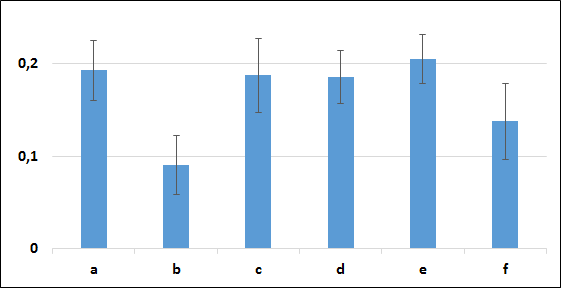
\includegraphics[width=8.5cm]{Pictures/PrivFixedMetric1.png}
      \caption{Number of events handled per time unit for the private, fixed-thresholds algorithms with different thresholds $\theta$ and steepnesses $n$. (a) $\theta=5, n=+\infty$, (b) $\theta=8, n=+\infty$, (c) $\theta=5, n=10$, (d) $\theta=8, n=10$, (e) $\theta=5, n=30$, (f) $\theta=8, n=30$.}
      \label{figure1}
   \end{figure}
	 \begin{figure}[thpb]
      \centering
      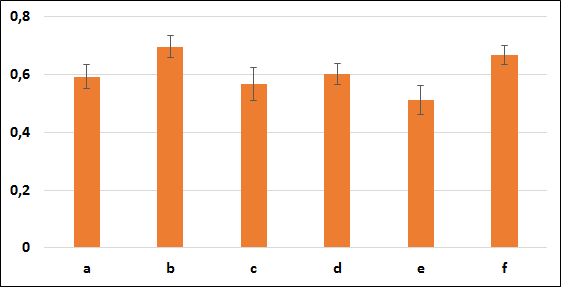
\includegraphics[width=8.5cm]{Pictures/PrivFixedMetric2.png}
      \caption{Second metric for the private, fixed-thresholds algorithms with different thresholds $\theta$ and steepnesses $n$. (a) $\theta=5, n=+\infty$, (b) $\theta=8, n=+\infty$, (c) $\theta=5, n=10$, (d) $\theta=8, n=10$, (e) $\theta=5, n=30$, (f) $\theta=8, n=30$.}
      \label{figure2}
   \end{figure}
	\begin{figure}[thpb]
      \centering
      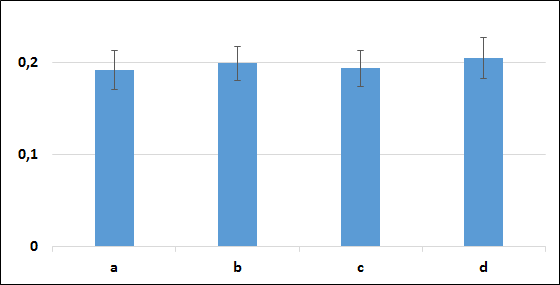
\includegraphics[width=8.5cm]{Pictures/PrivAdaptMetric1.png}
      \caption{Number of events handled per time unit for the private, adaptive-thresholds algorithms with a steepness $n=30$ and different thresholds $\theta$ and adaptation factors $\delta_{\theta}$. (a) $\delta_{\theta}=0.1$, (b) $\delta_{\theta}=0.01$, (c) $\delta_{\theta}=0.1$(d) $\delta_{\theta}=0.01$.}
      \label{figure3}
   \end{figure}
	\begin{figure}[thpb]
      \centering
      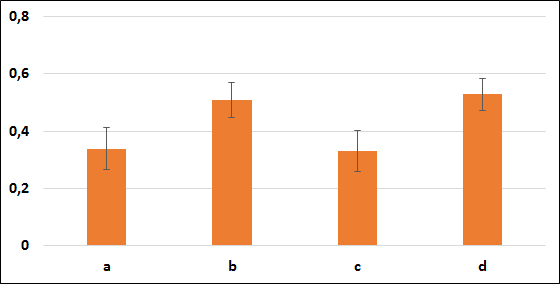
\includegraphics[width=8.5cm]{Pictures/PrivAdaptMetric2.png}
      \caption{Second metric for the private, adaptive-thresholds algorithms with a steepness $n=30$ and different thresholds $\theta$ and adaptation factors $\delta_{\theta}$. (a) $\delta_{\theta}=0.1$, (b) $\delta_{\theta}=0.01$, (c) $\delta_{\theta}=0.1$(d) $\delta_{\theta}=0.01$.}
      \label{figure4}
   \end{figure}
	\begin{figure}[thpb]
      \centering
      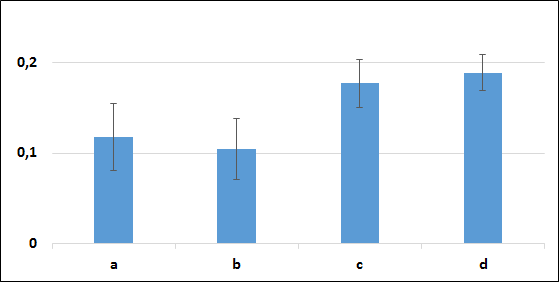
\includegraphics[width=8.5cm]{Pictures/PrivSpecMetric1.png}
      \caption{Number of events handled per time unit for the private, adaptive-thresholds with specialization algorithms with a steepness $n=30$, an initial threshold of $\theta=5$ and different specialization rates. (a) Specialization rate $-1/+1$ and no adaptation, (b) Specialization rate $-1/+2$ and no adaptation, (c) Specialization rate -0.5/+0.5 and adaptation $\delta_{\theta}=0.01$, (d) Specialization rate -1/+1 and adaptation $\delta_{\theta}=0.01$.}
      \label{figure5}
   \end{figure}
	\begin{figure}[thpb]
      \centering
      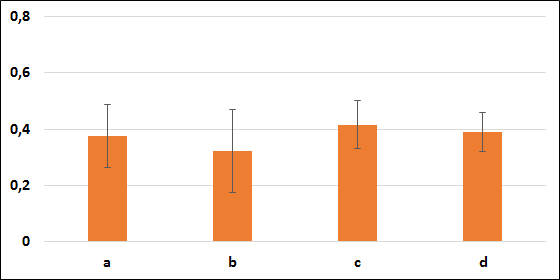
\includegraphics[width=8.5cm]{Pictures/PrivSpecMetric2.png}
      \caption{Second metric for the private, adaptive-thresholds with specialization algorithms with a steepness $n=30$, an initial threshold of $\theta=5$ and different specialization rates. (a) Specialization rate $-1/+1$ and no adaptation, (b) Specialization rate $-1/+2$ and no adaptation, (c) Specialization rate -0.5/+0.5 and adaptation $\delta_{\theta}=0.01$, (d) Specialization rate -1/+1 and adaptation $\delta_{\theta}=0.01$.}
      \label{figure6}
   \end{figure}
	\begin{figure}[thpb]
      \centering
      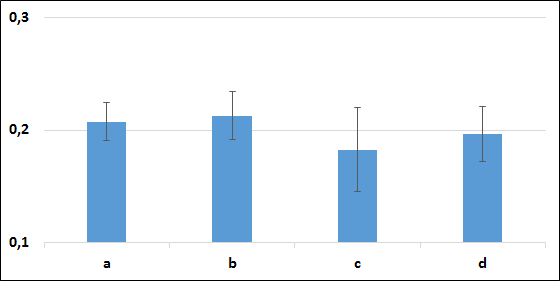
\includegraphics[width=8.5cm]{Pictures/PubMetric1.png}
      \caption{Number of events handled per time unit for the public, adaptive-thresholds algorithms with $\alpha=1$, $n=\infty$, a communication range of 40cm and different values of $\beta$. (a) $\beta=0.1$ and adaptation $\delta_{\theta}=0.01$, (b) $\beta=0.2$ and adaptation $\delta_{\theta}=0.01$, (c) $\beta=0.1$ and no adaptation, (d) $\beta=0.2$ and no adaptation.}
      \label{figure7}
   \end{figure}
	\begin{figure}[thpb]
      \centering
      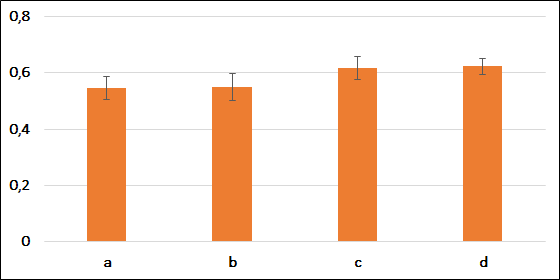
\includegraphics[width=8.5cm]{Pictures/PubMetric2.png}
      \caption{Second metric for the public, adaptive-thresholds algorithms with $\alpha=1$, $n=\infty$, a communication range of 40cm and different values of $\beta$. (a) $\beta=0.1$ and adaptation $\delta_{\theta}=0.01$, (b) $\beta=0.2$ and adaptation $\delta_{\theta}=0.01$, (c) $\beta=0.1$ and no adaptation, (d) $\beta=0.2$ and no adaptation.}
      \label{figure8}
   \end{figure}
